%
% related-work.tex
%
% Copyright (C) 2022 by SpaceLab.
%
% Camera Payload Preliminary Design Review
%
% This work is licensed under the Creative Commons Attribution-ShareAlike 4.0
% International License. To view a copy of this license,
% visit http://creativecommons.org/licenses/by-sa/4.0/.
%

%
% \brief Introduction slides.
%
% \author Gabriel Mariano Marcelino <gabriel.mm8@gmail.com>
% \author Vitória Beatriz Bianchin <vitoriabbianchin@gmail.com>
% \author Caique Sales de Miranda Gomes <kiqsmg@gmail.com>
%
% \version 0.1.0
%
% \date 2022/06/24
%


\begin{frame}{Comercial ADCS modules for CubeSats}

    A few commercial ADCS modules for CubeSats are available in the market:

    \begin{itemize}
        \item \href{https://www.isispace.nl/product/isis-magnetorquer-board/}{\textcolor{blue}{\underline{ISIS - iMTQ Magnetorquer Board}}}
        \vspace{0.4cm}
        \item \href{https://gomspace.com/shop/subsystems/attitude-orbit-control-systems/nanotorque-gst-600.aspx}{\textcolor{blue}{\underline{GomSpace - NanoTorque GST-600}}}
        \vspace{0.4cm}
        \item \href{https://nanoavionics.com/cubesat-components/cubesat-magnetorquer-satbus-mtq/}{\textcolor{blue}{\underline{NanoAvionics - CubeSat Magnetorquer SatBus MTQ}}}
        \vspace{0.4cm}
        \item \href{}{\textcolor{blue}{\underline{...}}}
    \end{itemize}

\end{frame}

% #########################################################################
% #########################################################################

\begin{frame}{Comercial ADCS: \href{https://www.isispace.nl/product/isis-magnetorquer-board/}{\textcolor{cyan}{\underline{ISIS - iMTQ Magnetorquer Board}}}}

    \begin{columns}[t]
        \begin{column}[t]{0.5\textwidth}
            \begin{itemize}
                \item Three-axis actuators: two magnetorquers with magnetic core and one with air core; Nominal dipole strength: $0.2 Am^2$;
                \item Current and temperature sensors for each magnetorquer;
                \item Suitable to detumble up to 12U (~24kg) CubeSats.
            \end{itemize}
        \end{column}
        \begin{column}[t]{0.5\textwidth}
            \begin{figure}[!ht]
                \begin{center}
                    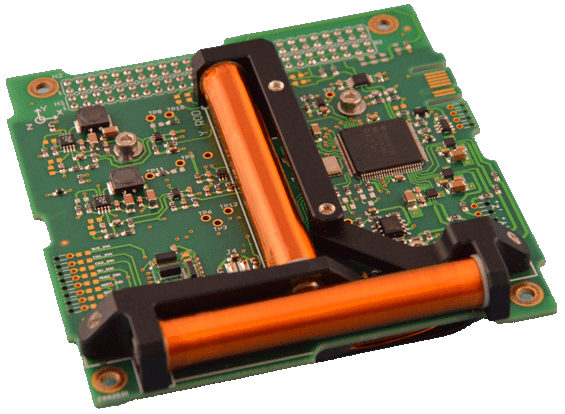
\includegraphics[width=4.5cm]{figures/magnetorquers-isis.png}
                \end{center}
            \end{figure}
        \end{column}
    \end{columns}

    

    
\end{frame}

\begin{frame}{Comercial Coils: \href{https://gomspace.com/shop/subsystems/attitude-orbit-control-systems/nanotorque-gst-600.aspx}{\textcolor{cyan}{\underline{GomSpace - NanoTorque GST-600}}}}

    \begin{columns}[t]
        \begin{column}[t]{0.5\textwidth}
            \begin{itemize}
                \item 3-axis magnetorquer;
                \item Torque $>0.3 Am^2$ per axis;
                \item Build-in temperature sensor;
                \item High torque and low residual dipole.
            \end{itemize}
        \end{column}
        \begin{column}[t]{0.5\textwidth}
            \begin{figure}[!ht]
                \begin{center}
                    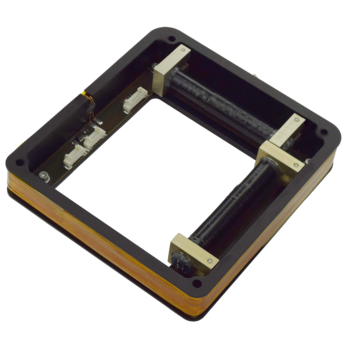
\includegraphics[width=4.5cm]{figures/magnetorquers-gomspace.png}
                \end{center}
            \end{figure}
        \end{column}
    \end{columns}
    
\end{frame}

% #########################################################################
% #########################################################################

\begin{frame}{Comercial Coils: \href{https://nanoavionics.com/cubesat-components/cubesat-magnetorquer-satbus-mtq/}{\textcolor{cyan}{\underline{NanoAvionics - CubeSat Magnetorquer MTQ}}}}

    \begin{columns}[t]
        \begin{column}[t]{0.5\textwidth}
            \begin{itemize}
                \item 2 magnetorquer rods with soft magnetic cores and 1 coil with air core;
                \item Dipole magnetic moment strength: $0.3 Am^2$ (X/Y axis), $0.34 Am^2$ (Z axis);
                \item Supply voltage: up to 5 V;
                \item Power consumption: 0.4 W.
            \end{itemize}
        \end{column}
        \begin{column}[t]{0.5\textwidth}
            \begin{figure}[!ht]
                \begin{center}
                    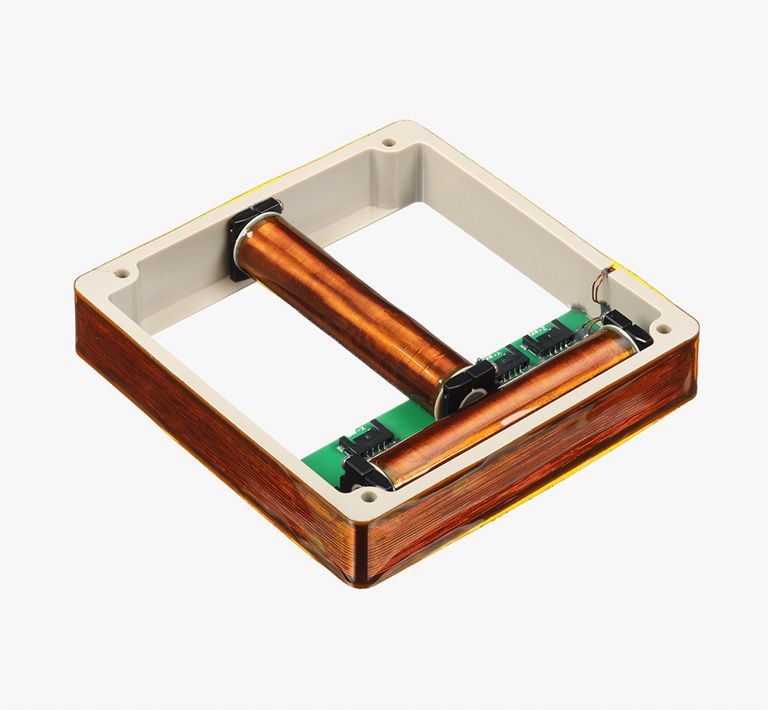
\includegraphics[width=4.5cm]{figures/magnetorquers-nanoavionics.png}
                \end{center}
            \end{figure}
        \end{column}
    \end{columns}
    
\end{frame}